\documentclass[12pt]{report}
\usepackage[utf8]{inputenc}
\usepackage[T1]{fontenc}
\usepackage{graphicx}
\usepackage{float}
\usepackage{listings}
\usepackage{xcolor}
\usepackage{hyperref}

\hypersetup{
    colorlinks=true,
    linkcolor=blue,
    urlcolor=blue,
    pdftitle={Group: Power Puff - Step 1},
    pdfauthor={Zainab Khan, Jade Wilson},
}

\lstset{
    language=Verilog,
    basicstyle=\ttfamily\footnotesize,
    keywordstyle=\color{blue},
    commentstyle=\color{gray},
    stringstyle=\color{red},
    numbers=left,
    numberstyle=\tiny,
    stepnumber=1,
    numbersep=5pt,
    breaklines=true,
    tabsize=2,
    showstringspaces=false,
}

\title{Group: Power Puff - Step 1: Verilog \& LaTeX Basics}
\author{Group Members: Zainab Khan and Jade Wilson}
\date{\today}

\begin{document}

\maketitle
\tableofcontents
\newpage

\chapter{Introduction}

This report summarizes the implementation and simulation of several 1-bit logic gates and a 1x4-bit arithmetic shift circuit using Verilog. The gates implemented include NOT, NAND, and NOR gates. We tested each circuit by running testbenches and verified their behavior using waveform simulations in GTKWave. Screenshots of the waveforms are included in the figures section.

\chapter{NOT Gate Implementation}

The NOT gate is a fundamental logic gate that outputs the logical negation of its single input.

\section{Verilog Code}

\lstinputlisting[language=Verilog]{Verilog/not_1b.v}

\section{Testbench}

\lstinputlisting[language=Verilog]{Verilog/not_1b_test.v}

\section{Waveform Results}

Figure~\ref{fig:not_waveform} shows the waveform output for the NOT gate. At 0 ns, input \texttt{a} is 0, resulting in output \texttt{y} being 1. This confirms the expected inversion behavior.

\begin{figure}[H]
    \centering
    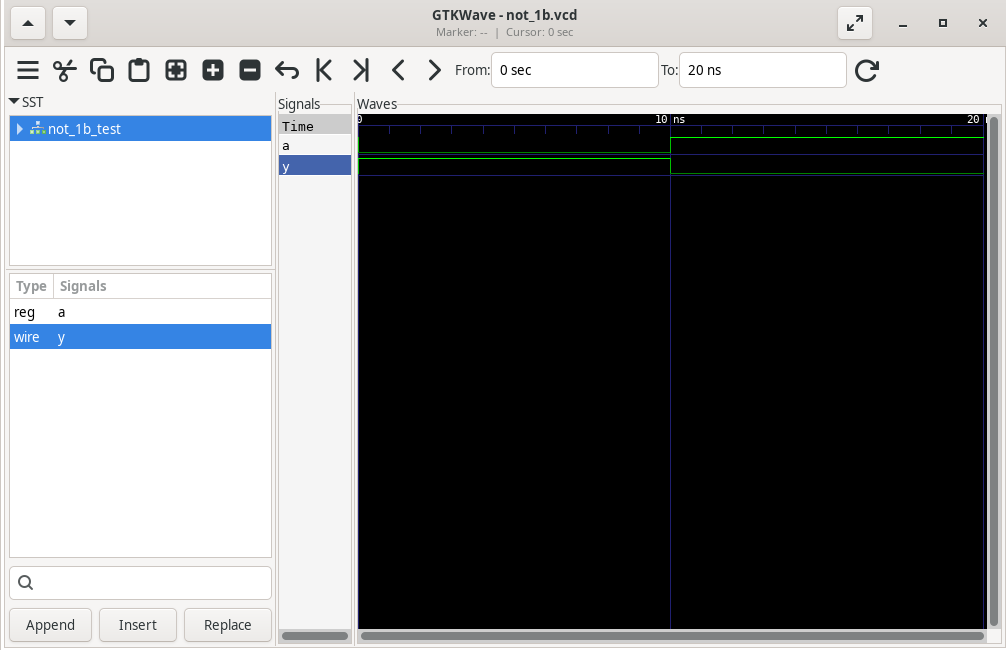
\includegraphics[width=1.0\textwidth]{figs/NOT_GATE_WAVEFORM.png}
    \caption{NOT Gate Waveform captured in GTKWave}
    \label{fig:not_waveform}
\end{figure}

\chapter{NAND Gate Implementation}

The NAND gate outputs the negation of the AND operation on two inputs.

\section{Verilog Code}

\lstinputlisting[language=Verilog]{Verilog/nand_1b.v}

\section{Testbench}

\lstinputlisting[language=Verilog]{Verilog/nand_1b_test.v}

\section{Waveform Results}

Figure~\ref{fig:nand_waveform} displays the simulation waveform for the NAND gate. The output correctly reflects the NAND logic for all input combinations.

\begin{figure}[H]
    \centering
    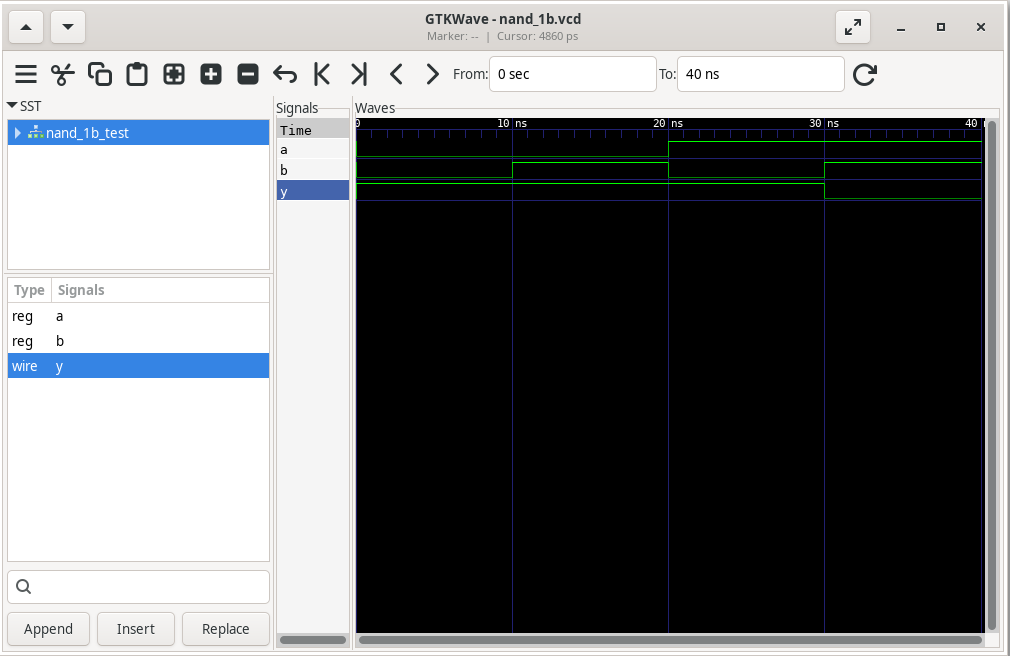
\includegraphics[width=1.0\textwidth]{figs/NAND_GATE_WAVEFORM.png}
    \caption{NAND Gate Waveform captured in GTKWave}
    \label{fig:nand_waveform}
\end{figure}

\chapter{NOR Gate Implementation}

The NOR gate outputs the negation of the OR operation on two inputs.

\section{Verilog Code}

\lstinputlisting[language=Verilog]{Verilog/nor_1b.v}

\section{Testbench}

\lstinputlisting[language=Verilog]{Verilog/nor_1b_test.v}

\section{Waveform Results}

Figure~\ref{fig:nor_waveform} shows the waveform simulation for the NOR gate. The output confirms the NOR truth table.

\begin{figure}[H]
    \centering
    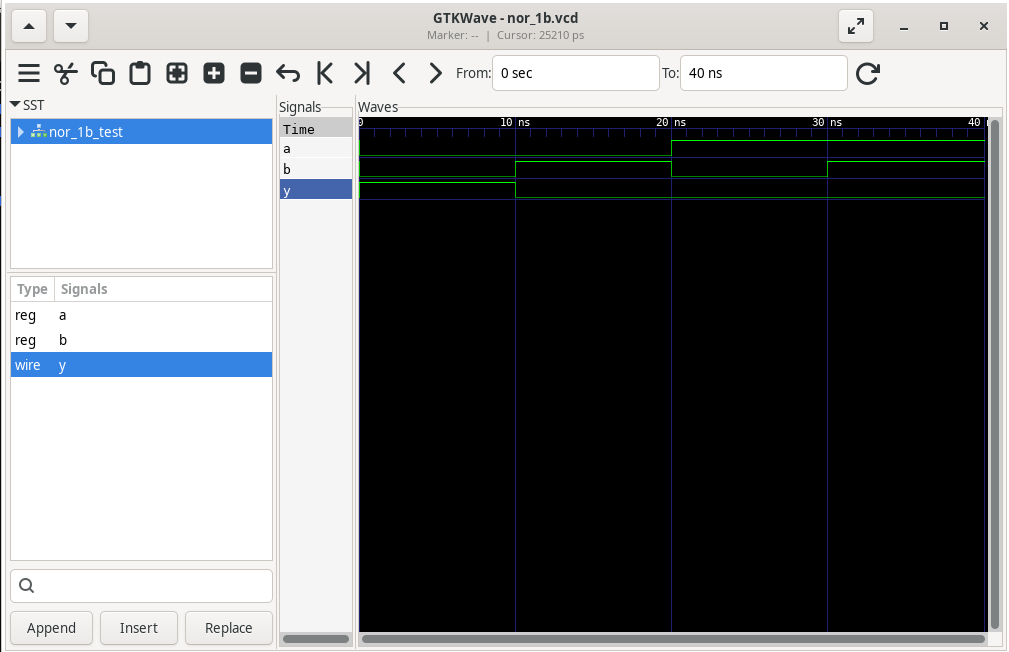
\includegraphics[width=1.0\textwidth]{figs/NOR_GATE_WAVEFORM.png}
    \caption{NOR Gate Waveform captured in GTKWave}
    \label{fig:nor_waveform}
\end{figure}

\chapter{1x4-bit Arithmetic Shift Circuit}

This circuit performs an arithmetic shift operation on a 4-bit input, shifting bits either left or right.

\section{Verilog Code}

\lstinputlisting[language=Verilog]{Verilog/shift_4b.v}

\section{Testbench}

\lstinputlisting[language=Verilog]{Verilog/shift_4b_test.v}

\section{Waveform Results}

Figure~\ref{fig:shift_waveform} shows the waveform simulation for the 1x4-bit arithmetic shift circuit.

\begin{figure}[H]
    \centering
    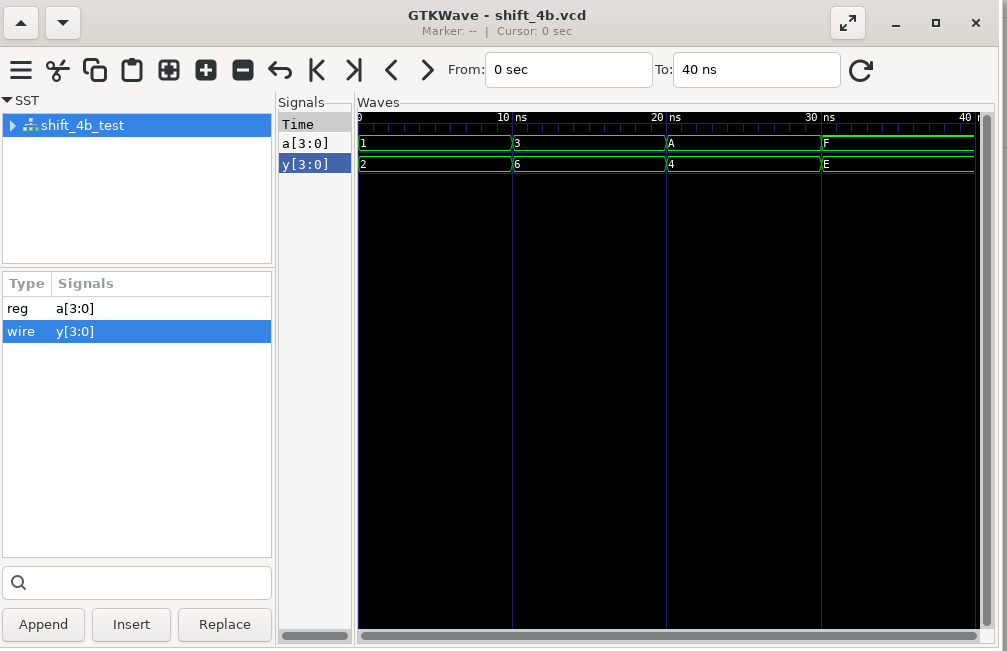
\includegraphics[width=1.0\textwidth]{figs/SHIFT_WAVEFORM.png}
    \caption{1x4-bit Arithmetic Shift Circuit Waveform captured in GTKWave}
    \label{fig:shift_waveform}
\end{figure}

\chapter{Conclusion}

We have successfully implemented and tested basic logic gates (NOT, NAND, NOR) and a 1x4-bit arithmetic shift circuit using Verilog. Testbenches were used to verify functionality, and waveform simulations confirmed correct operation of each circuit. This step establishes the foundation for more complex designs in future project steps.

\end{document}

